\documentclass[12pt,a4paper]{article}

\usepackage{amssymb}
\usepackage[T1]{fontenc}
\usepackage[utf8]{inputenc}
\usepackage[polish]{babel}
\usepackage{indentfirst}
\usepackage{amsfonts}
\usepackage{amsmath}
\usepackage{algorithmic}

\usepackage[margin=0.5in,headheight=48pt,top=78pt]{geometry}
\frenchspacing
\setlength{\parskip}{1em}
\setlength{\parindent}{0em}
\def\N{\mathbb{N}}
\def\R{\mathbb{R}}
\newcommand{\zadanie}[1]{\par\textbf{Zadanie #1}}
\newcommand{\odp}[1]{\textbf{Odpowiedź:} #1}

\usepackage{tikz}

\usepackage{fancyhdr}
\pagestyle{fancy}
\fancyhf{} % clear all fields
\fancyhead[C]{ \textbf{SK} - Pracowania 7\ Wiktor Pilarczyk 308533}

\begin{document}
Maszyna została skonfigurowana zgodnie z zaleceniami dla obu zadań.

\zadanie{1}
Na maszynie Virbian2 strumień danych występuje w postaci niezaszyfrowanej jako
pakiety przesyłane z ::1 port 22 do ::1 port 34796 poprzez IPv6.
\begin{figure}[!htb]
\centering
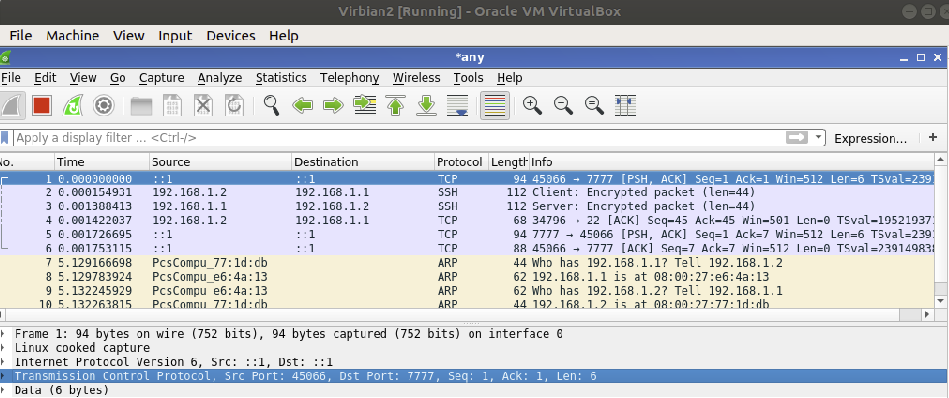
\includegraphics[scale=0.3]{a.png}
\caption{Strumień danych w V2 w postaci niezaszyfrowanej}
\end{figure}

Pomiędzy maszyną Virbian2 a maszyną Virbian1 strumień danych występuje w postaci zaszyfrowanej jako pakiety przesyłane z 192.168.1.2 port 34796 do 192.168.1.1 port 22 poprzez IPv4.

\begin{figure}[!htb]
\centering
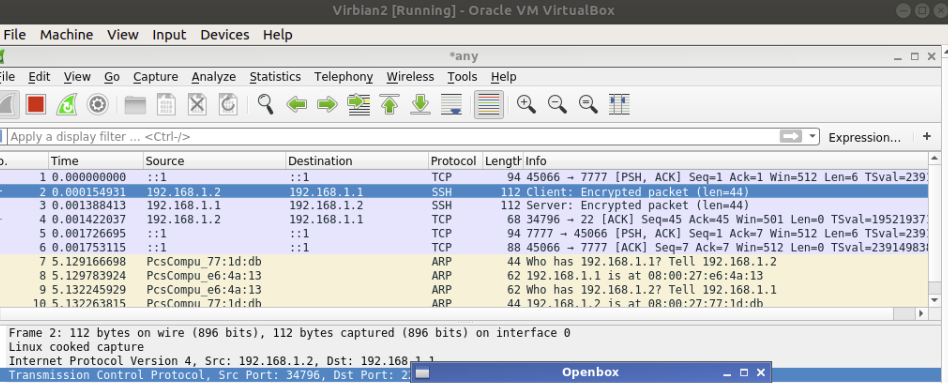
\includegraphics[scale=0.3]{b.png}
\caption{Strumień danych V2 pomiędzy V1 w postaci zaszyfrowanej (trochę się ucieło)}
\end{figure}

Na maszynie Virbian1 strumień danych występuje w postaci niezaszyfrowanej jako
pakiety przesyłane z 127.0.0.1 port 34796 do 127.0.0.1 port 7 poprzez IPv4.
\begin{figure}[!htb]
\centering
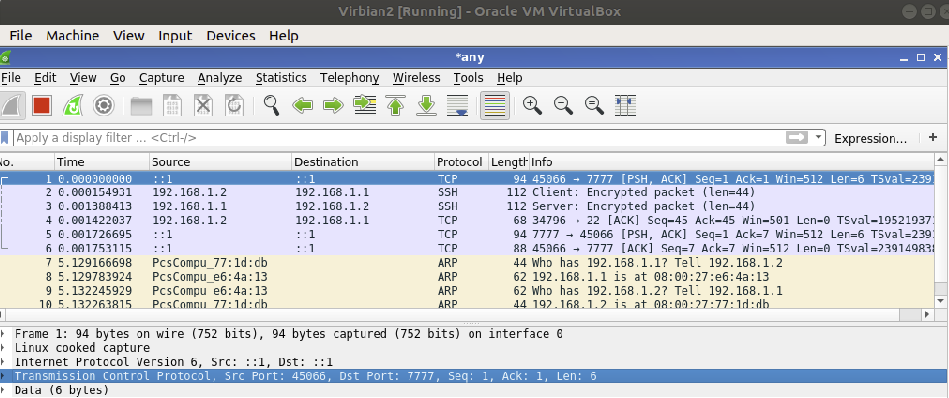
\includegraphics[scale=0.3]{a.png}
\caption{Strumień danych w V1 w postaci niezaszyfrowanej}
\end{figure}

\zadanie{2} Opiszę tylko komendy, które nie zostały podane.

Za pomocą komendy ,,gpg --gen-key" generuje klucz prywatny dla user2 i powtarzam komende eksportującą tylko dla user2.

Za pomocą komendy ,,scp 192.168.1.1:user1-pgp-key user1-pgp-key" kopiuje klucz user1 na maszynę V2.

Aby wejść w tryb edycji klucza i upewnić się, że jego funkcja skrótu i podpisanie w następujących krokach:

\begin{enumerate}
\item gpg --edit-key user1@mail.example.com
\item fpr
\item Funkcje skrótu sprawdzam po prostu skrót klucza na V1 i V2.
\item sign i quit
\end{enumerate}
\begin{figure}[!htb]
\centering
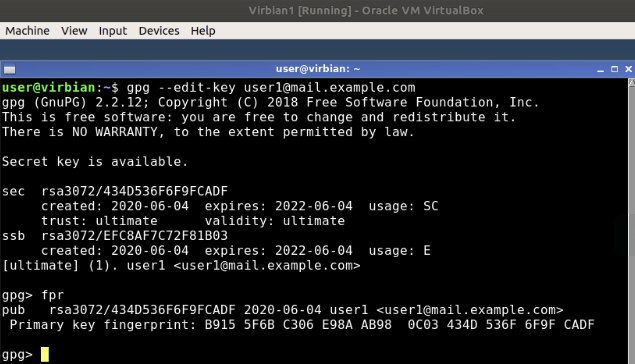
\includegraphics[scale=0.4]{V1key.png}
\caption{Klucz na maszynie V1}
\end{figure}
\begin{figure}[!htb]
\centering
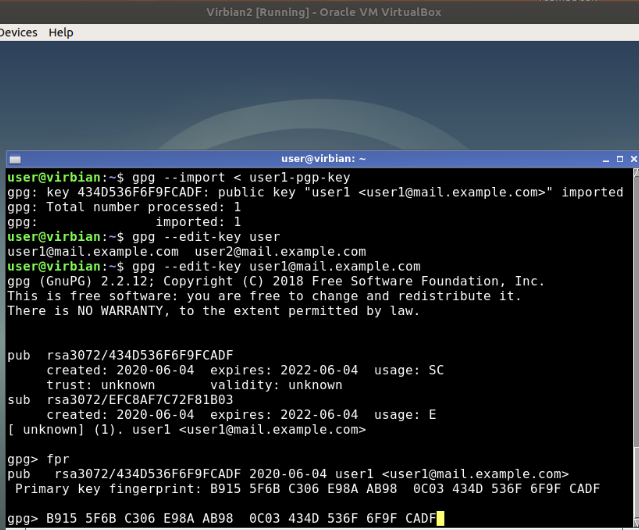
\includegraphics[scale=0.4]{V2key.png}
\caption{Klucz na maszynie V2}
\end{figure}
Następnie konfiguruje ssh na V2 i wykonuje podobne instrkucje, ale dla V1.

Tworzę plik message za pomocą:
\begin{enumerate}
\item touch message
\item echo halo > message
\end{enumerate}
Następnie szyfruje, a następnie kopiuje na V2 za pomocą instrukcji "scp message.asc 192.168.1.2:message.asc".
\begin{figure}[!htb]
\centering
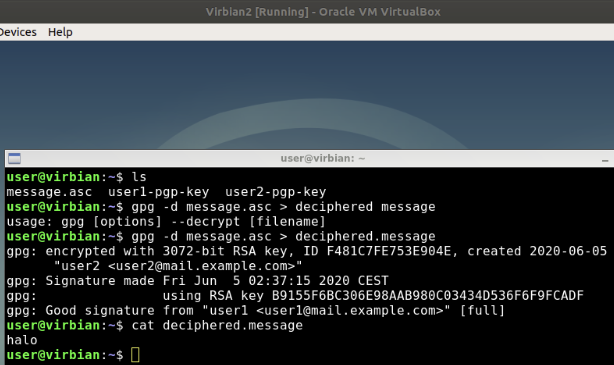
\includegraphics[scale=0.6]{message.png}
\caption{Rozszyfrowana wiadomość}
\end{figure}
\end{document}
